\fontsize{12bp}{14bp}\selectfont
\subsection{Motivation} 
The motivation for this paper could be best illustrated by the following two maps:\footnote{Source: http://www.cdc.gov/obesity/data/adult.html}\footnote{Source: http://www.zook.info/Wal-Mart/Figure2-2-US-distribution-by-store-type.jpg}

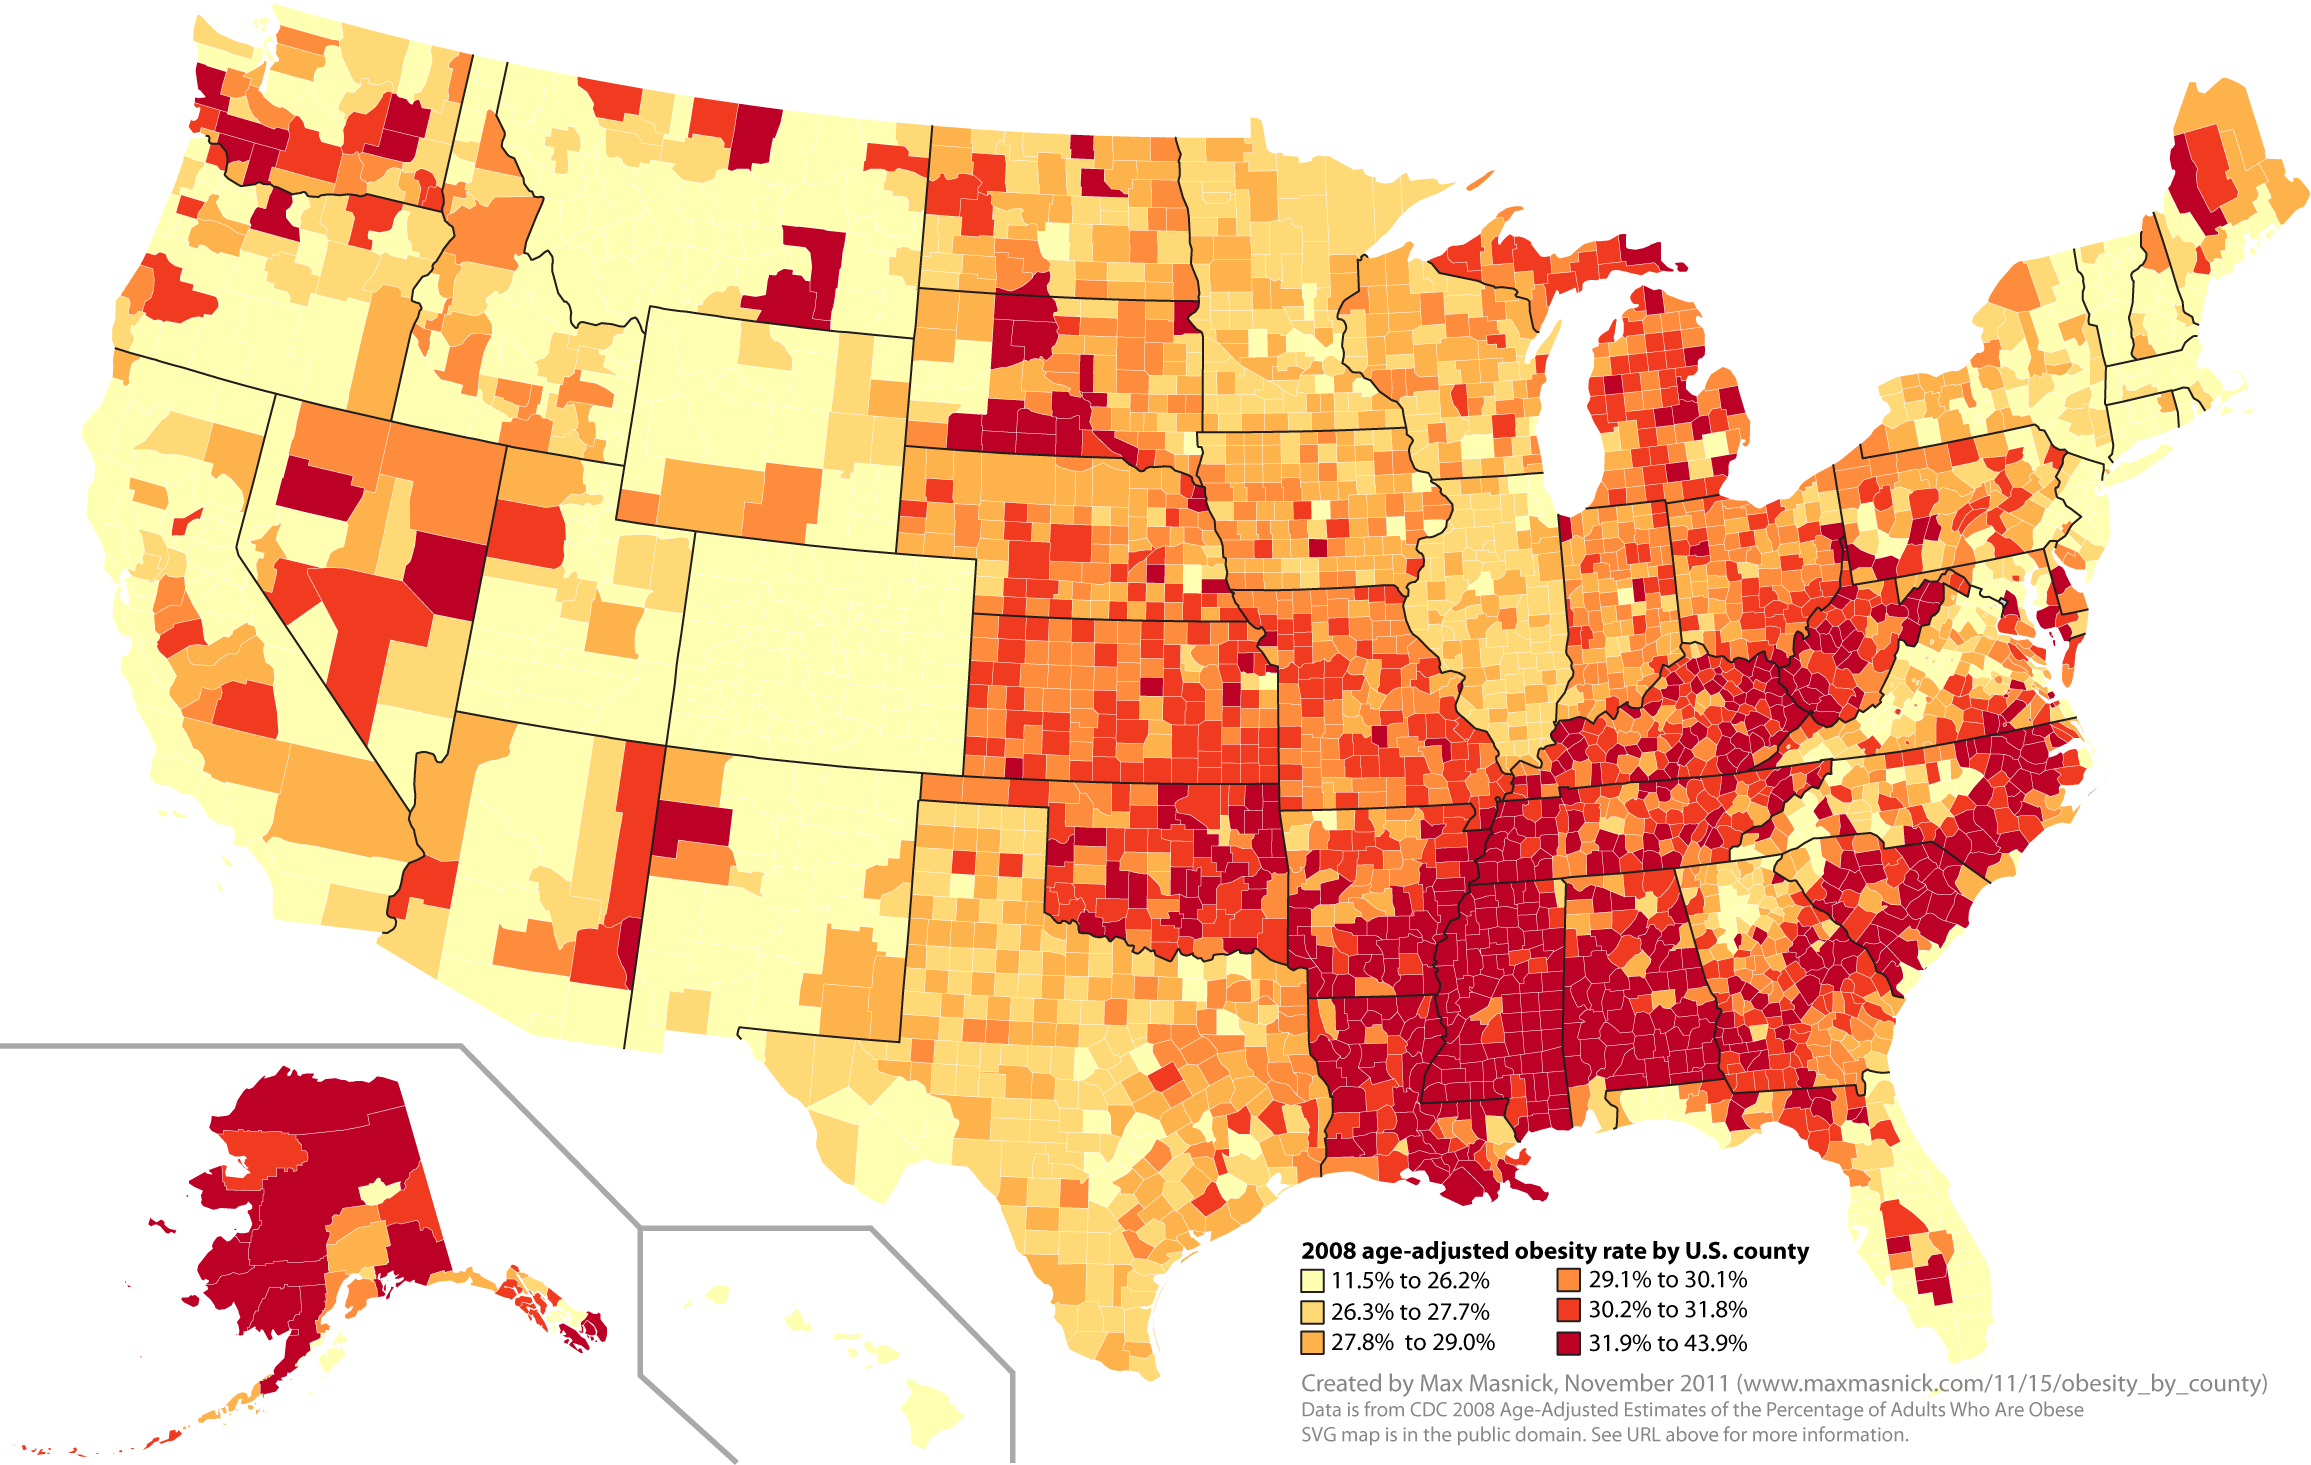
\includegraphics[width=200px]{obesity_by_county_large}
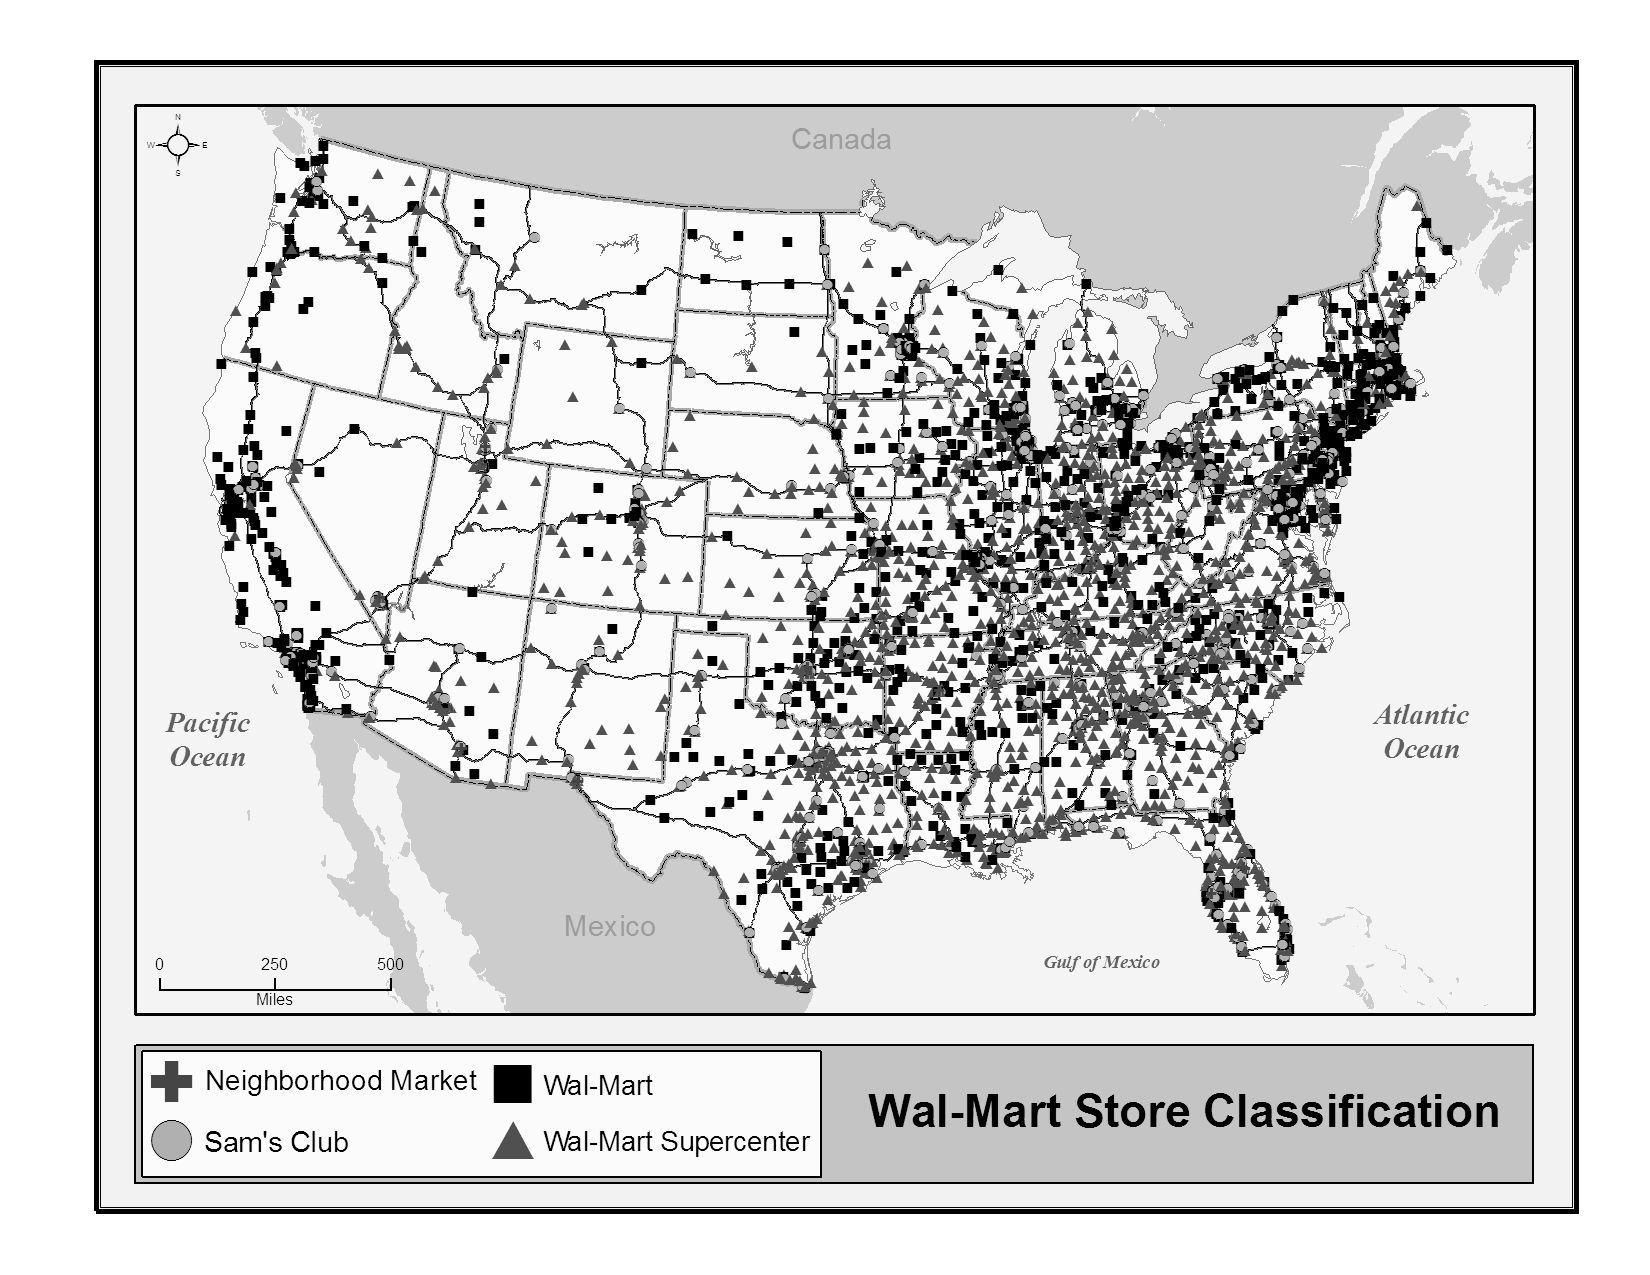
\includegraphics[width=200px]{walmartdistribution}

At first glance, there appears to be a clear correspondence between the density of Wal-Mart stores and the rate of obesity for a given area.  The match is imperfect and the actual relationship, if any, cannot be gleaned from these images alone but it does provide adequate motivation for us to explore the quality and degree of their relationship through econometric methods.  Although not shown here because of space constraints, the pattern of correspondence appears to hold over time as well.  
\subsection{Obesity}

The definition of obesity varies, but a Body-Mass-Index (BMI) of 30 kg/m is a typical value for differentiating those who are obese from those who are not.  Using this criteria, 78 million adults and 12.5 million children in the United States are obese.  A person with a BMI between 30 and 35 can expect to pay \$1850 more per year in medical expenses than a non-obese person, between 35 and 40 the cost rises to \$3086 more per year and \$5530 per year for those with a BMI above 40.  For comparison, those who smoke pay \$1274 per year more than non-smokers.\footnote{Sharon Begley. The Costs of Obesity. Huffington Post. 30 APR 2012}  Further, obesity is linked to high blood pressure, diabetes, stroke and heart disease. \footnote{Charles Courtemanche. Supersizing Supercenters? The Impact of Wal-Mart Supercenters on Body Mass Index and Obesity. Journal of Urban Economics, Elsevier, vol. 69(2), pages 165-181, March.} The Mayo clinic lists the following as risk factors for obesity:  genetics, lifestyle, diet, smoking, pregnancy, lack of sleep, medications, age, socioeconomic factors, and medical problems.\footnote{Source: http://www.mayoclinic.com/health/obesity/DS00314/DSECTION=risk-factors}  
\subsection{Wal-Mart Stores, Inc.}

The first Wal-Mart store opened in Rogers, Arkansas in 1962. By focusing on dominating the retail space in towns with less than 50 thousand people, Wal-Mart grew to become the nation's largest retailer in 1990.  Three years later, the company had its first "billion dollar week."  It topped the Fortune 500 list for the first time in 2002 and now has 2.2 million employees, 200 million customers per week and more than 10,000 stores world-wide.\footnote{Source: http://corporate.walmart.com/our-story/heritage/history-timeline} In 1988, Wal-Mart opened the first "Supercenter" which included full service groceries.

The opening of a Wal-Mart store has a number of complex, interacting economic consequences and the net effect is truly difficult to quantify.  In rural areas, Wal-Mart's deeply discounted prices and the variety of products available for sale may truly be a boon for the local economy.  In many cases, retail sales are being reallocated - as much as 25 million dollars annually - from other businesses, many of which close or downsize.  Over the course of twenty years, the local economy may produce as much as 13 million dollars less in total output.\footnote{David Mielach. What It Really Costs When Wal-Mart Comes to Town. Businessweek Daily. 23 Apr 2012.}

Certainly, the decisions Wal-Mart makes in selecting products for its shelves has an impact multiplied over its hundreds of millions of customers per week.